\section{Aritmetické operace v počítači}
\label{sec:aritmeticke-operace}
Aritmetické operace v počítači zahrnují součet, rozdíl, součin a podíl.
Provádění těchto operací provádí ALU.
Mimo aritmetických operací se ALu stará i o operace logické (AND, OR, NOT,\dots).
Racionální číslo je takové číslo, které lze zapsat jako zlomek.
Všechny počítače provádějí operace v binární soustavě.
Všechny operace se převádí na určitou formu sčítání nebo násobení pro výpočet.
\subsection{Ukládání desetinných čísel}
Pro zobrazení reálných, velmi malých a nebo velmi velkých číšel se používá pohyblivá řádka.
Formát takového čísla bývá: $x = M*z^E$.
M = mantissa, E = exponent (v obrázku "fraction"), z = základ (2), x = výsledek.
K jeho zápisu nám slouží \textbf{Single precision formát}, která ukladá tyto hodnoty ve 4 bajtech paměti.\\

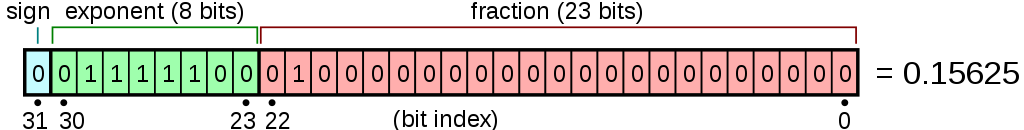
\includegraphics[width=\linewidth]{TVY-POS/Ciselne-soustavy/single_precision.png}\\

Základ čísla se neukládá, ale místo něho můžeme na posledním bitu vidět znaménkový bit pro určení záportného čísla.
Exponent se ukladá ve tvaru od -126 do 127, kde hodnota 128 představuje nulu.
Hodnoty -127 (Samé 0) a 128 (Samé 1) jsou používány pro speciální čísla (nenašel jsem).
Existují také další precision formáty, které ukládají čísla na větší místo v paměti (64bit, 128bit) určené pro přesnější čísla.

\subsection{Sčítání}
Stejné jako v desítkové soustavě.
Pod sebou se sčítají čísla o stejných řádech.
$1011 + 1011 = 10110$

\subsection{Rozdíl}
Odčítání se převádí na formu sčítání pomocí dopňkového kódu.
První číslo zůstane beze změny $1011$.
Druhé číslo nejdříve projde inverzí $0101 \rightarrow 1010$, poté se k němu přičte $+1 \rightarrow 1101$.
Tyto dvě čísla poté sečteme a zkrátíme na původní délku čísel $1011 + 1011 = 10110 \rightarrow 0110$.

\subsection{Sčítání a rozdíl v pohyblivé čárce}
\begin{enumerate}
  \item Nejdříve provádí kontrola čísel, zdali se nejedná například o dělení nulou, nebo o NaN.
  \item Dále se určuje která číslo je větší.
  \item Znaménkový bit určuje větší číslo.
  \item Poté se porovnají exponenty obou čísel.
  \item Jestliže exponenty čísel nejsou stejné, tak vypočítá jejich rozdíl jako exponent výsledku.
  \item Mantisa menšího čísla se posune doprava o počet bitů rozdílu exponenů
  \item Jestliže výsledek přeteře, tak se výledek vrátí jako nekonečno
  \item Jestliže podteče, tak je výsledek buďto kladná nebo záporná nula
\end{enumerate}

\subsection{Součin}
Násobení se provádí stejně jako při počítání na papíře.
Tím pádem se oprace převede na formu sčítání a shiftování.
Nebo se využívá akcelerované verze při násobení a dělení dvojkou pomocí pohyblivé čárky.
$1001 (9) * 10 (2) = 10010 (18)$
\subsection{Podíl}
Tato operace je velmi složitá pro počítač a proto se převádí například na postupné odečítání dělitele od dělence nebo posunem destiné čárky.
$1001 (9) : 10 (2) = 100.1 (4.5)$
\begin{center}
  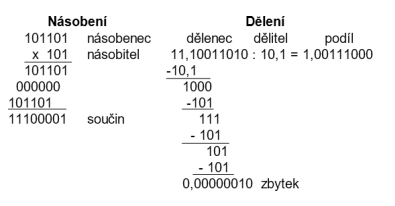
\includegraphics[width=0.5\linewidth]{TVY-POS/Aritmeticke-operace/nasobeni-deleni.png}
\end{center}
